\documentclass[11pt,a4paper]{article}
\usepackage[utf8]{inputenc}
\usepackage[margin=1in]{geometry}
\usepackage{amsmath,amssymb,amsfonts}
\usepackage{booktabs}
\usepackage{graphicx}
\usepackage{hyperref}
\usepackage{listings}
\usepackage{xcolor}

\newcommand{\discussionnote}[1]{\textcolor{blue}{\scriptsize\emph{(#1)}}}

\title{\textbf{Concept Mapping Algorithm Benchmarking Framework}}
\author{}
\date{\today}

\begin{document}

\maketitle

\begin{abstract}
Concept mapping combines qualitative statement sorting with quantitative multivariate analysis to model complex domains. However, comparing clustering algorithms requires a controllable reference model, because empirical concept mapping data do not provide an absolute ground truth. This document describes the current benchmark framework: the mathematical generation of synthetic similarity matrices, the progressive benchmark design, the evaluation metrics, and the interface for adding new algorithms.
\end{abstract}

\noindent\textbf{Repository:} \url{https://github.com/ruicdacosta/Concept-Mapping-Framework}

\vspace{0.5em}

\tableofcontents
\newpage

\section{Context and Motivation}

Concept mapping methodologies can be implemented through different analytical sequences. The traditional Trochim approach applies multidimensional scaling (MDS) followed by cluster analysis, whereas the P\'eladeau-type approach avoids the intermediate MDS projection and clusters directly on the original dissimilarity matrix. These approaches are mathematically different: one performs clustering after a dimensional reduction step, while the other works directly on the pairwise relations.

At the present stage, we do not know which algorithm performs better, nor under which types of problem complexity each method begins to fail. Empirical data are not sufficient for this question because the true clustering is not known. A synthetic benchmark is therefore needed: one where the true model is created first, the observed similarity matrix is generated from it, and each algorithm is evaluated by how well it reconstructs the original assignment structure.

\section{Goal}

The goal is to create a ``true'' model for concept mapping clustering problems. This true model is used to generate similarity matrices with controlled levels of ambiguity and noise. Since the ground-truth assignment matrix is known, different algorithms can be compared using the same input matrix \(S\) and the same expected number of clusters \(k\).

The framework is intended to support future methodological work. However, it does not yet define the final benchmark standard. \discussionnote{The final benchmark design still needs to be discussed and refined.}

\section{How: Mathematical Generation Pipeline}

The framework generates a synthetic concept mapping problem through a sequence of matrices. Let \(st\) be the number of statements and \(k\) the number of clusters.

\subsection{Ground-Truth Assignment Matrix}

The true statement-to-cluster structure is represented by a binary matrix
\[
Z \in \{0,1\}^{st \times k},
\]
where
\[
Z_{ia} =
\begin{cases}
1, & \text{if statement } i \text{ belongs to cluster } a,\\
0, & \text{otherwise.}
\end{cases}
\]
In the current implementation each statement belongs to exactly one cluster:
\[
\sum_{a=1}^{k} Z_{ia}=1, \qquad i=1,\ldots,st.
\]

\subsection{Cluster Similarity Matrix}

The cluster-level similarity structure is represented by a symmetric matrix
\[
C \in \mathbb{R}^{k \times k}.
\]
The diagonal entries \(C_{aa}\) describe within-cluster similarity and are sampled from
\[
C_{aa} \sim \mathcal{N}(\mu_{cii},\sigma_{cii}^{2}),
\]
whereas the off-diagonal entries \(C_{ab}\), \(a \neq b\), describe between-cluster similarity and are sampled from
\[
C_{ab} \sim \mathcal{N}(\mu_{cij},\sigma_{cij}^{2}).
\]
The matrix is made symmetric by imposing \(C_{ab}=C_{ba}\). Thus, \(C\) controls how distinct or overlapping the true clusters are before noise is added.

For illustration, consider the following cluster similarity matrices:
\[
C_1 =
\begin{bmatrix}
1 & 0 & 0\\
0 & 1 & 0\\
0 & 0 & 1\\
\end{bmatrix},
C_2 =
\begin{bmatrix}
0.9 & 0.2 & 0.5\\
0.2 & 0.9 & 0.1\\
0.5 & 0.1 & 0.9\\
\end{bmatrix},
C_3 =
\begin{bmatrix}
1 & 0.2 & 0.5\\
0.2 & 0.9 & 0.1\\
0.5 & 0.1 & 0.6\\
\end{bmatrix}
\]
These matrices induce increasingly different conceptual geometries. A schematic 2D representation is shown below:

\begin{figure}[ht!]
    \centering
    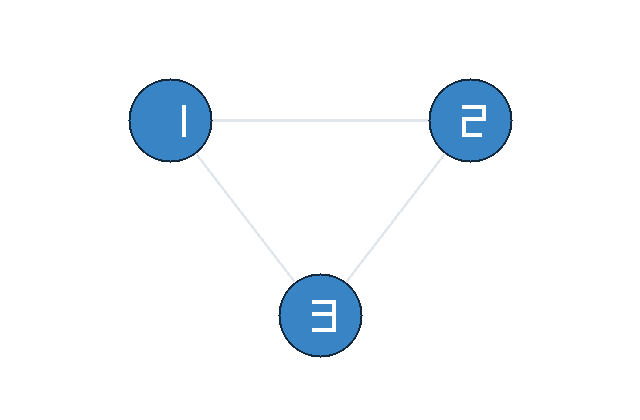
\includegraphics[width=0.3\linewidth]{figures/C_1.png}
    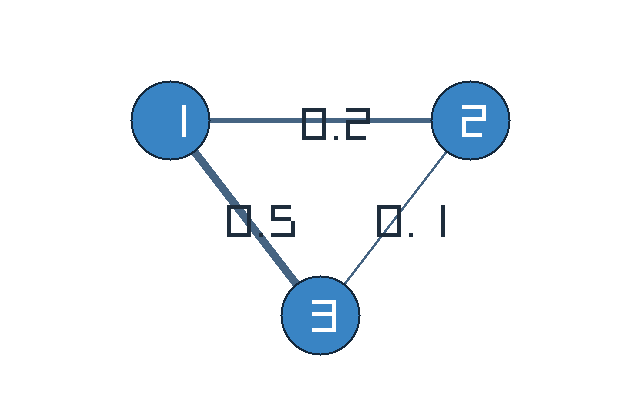
\includegraphics[width=0.3\linewidth]{figures/C_2.png}
    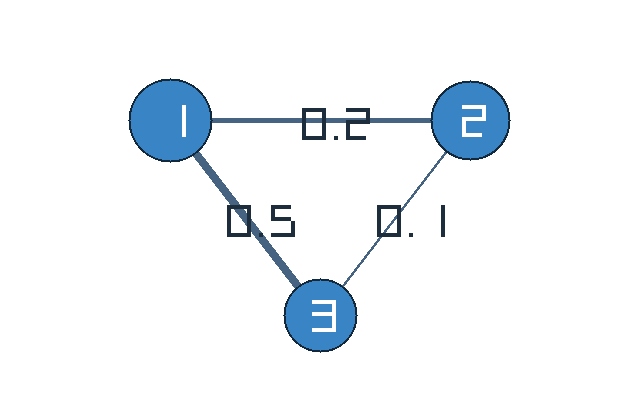
\includegraphics[width=0.3\linewidth]{figures/C_3.png}
    \caption{Schematic 2D illustrations of the cluster relations encoded by \(C_1\), \(C_2\), and \(C_3\). These plots are only visual aids; the benchmark itself uses the full matrix \(C\), not this two-dimensional representation.}
    \label{fig:c-illustrations}
\end{figure}

\subsection{Base Similarity Matrix}

The noise-free statement-level similarity matrix is computed as
\[
S_0 = Z C Z^\top .
\]
This equation is the core of the framework. If statement \(i\) belongs to cluster \(a\), and statement \(j\) belongs to cluster \(b\), then
\[
(S_0)_{ij}=C_{ab}.
\]
Therefore, \(Z\) defines which cluster each statement belongs to, and \(C\) defines the similarity assigned to each pair of clusters. The multiplication \(Z C Z^\top\) converts the cluster-level matrix \(C\) into a statement-level matrix \(S_0\).

\subsection{Error Matrix and Final Similarity Matrix}

To model human sorting disagreement and measurement noise, we generate a symmetric error matrix
\[
E \in \mathbb{R}^{st \times st},
\qquad
E_{ij} \sim \mathcal{N}(0,\sigma_e^{2}), \quad i<j,
\]
with \(E_{ij}=E_{ji}\) and \(E_{ii}=0\). The final observed similarity matrix is
\[
S = S_0 + E.
\]
The diagonal is then forced to
\[
S_{ii}=1,
\]
representing perfect self-similarity. The algorithms receive only \(S\) and \(k\). They do not receive \(Z\), \(C\), or \(S_0\).

\section{The Benchmark Framework (current state)}

The benchmark evaluates an algorithm over several generated problems rather than at a single fixed point. A run is organized into a sequence of difficulty steps. At each step, the framework generates a problem according to
\[
(st, k, \mu_{cii}, \sigma_{cii}, \mu_{cij}, \sigma_{cij}, \sigma_e).
\]
For each step, the algorithm is run several times, because the generation of \(Z\), \(C\), and \(E\) is stochastic.

The benchmark starts with well-defined clustering problems: high within-cluster similarity, low between-cluster similarity, low variability, and low noise. It then evolves toward more confusing problems by changing the parameters. The number of statements \(st\) may increase, the number of clusters \(k\) may increase, within-cluster similarity may decrease, between-cluster similarity may increase, the variability of \(C\) may increase, and the noise level \(\sigma_e\) may increase.

These changes affect different forms of complexity. Increasing \(k\) creates more competing clusters. Increasing \(\mu_{cij}\) reduces the contrast between clusters. Increasing \(\sigma_{cii}\) and \(\sigma_{cij}\) makes the cluster similarity structure less regular. Increasing \(\sigma_e\) corrupts the statement-level matrix after the true structure has been created. Eventually, the generated problem may become very ambiguous or even practically impossible to solve. The best algorithm should tend to maintain good metric values further along this difficulty evolution.

\section{Evaluation Metrics}

The predicted assignment matrix is denoted by
\[
Z_{\mathrm{alg}} \in \{0,1\}^{st \times k}.
\]
Because clustering labels are arbitrary, the columns of \(Z_{\mathrm{alg}}\) cannot be directly compared with the columns of \(Z\). The framework first solves the label permutation problem using the Hungarian algorithm, choosing the column alignment that maximizes overlap between true and predicted clusters.

After alignment, the matrices are converted into label vectors \(y\) and \(\hat{y}\). The current metrics are computed for each run.

\subsection{Accuracy}

\[
\mathrm{Accuracy}
=
\frac{1}{st}
\sum_{i=1}^{st}\mathbb{I}(y_i=\hat{y}_i).
\]
Accuracy measures the fraction of statements assigned to the correct aligned cluster. It is simple and interpretable, but it may be influenced by cluster-size imbalance. For example, if \(st=100\) and \(k=2\), with 90 statements in cluster 1 and 10 statements in cluster 2, an algorithm that assigns every statement to the largest cluster could still obtain a high accuracy value.

\subsection{Jaccard Coefficients}

For cluster \(a\), let \(T_a\) be the set of statements truly assigned to cluster \(a\), and \(P_a\) be the set of statements predicted to belong to cluster \(a\). The cluster-level Jaccard coefficient is
\[
J_a
=
\frac{|T_a \cap P_a|}{|T_a \cup P_a|}.
\]

The first Jaccard metric is
\[
\mathrm{Jaccard\_eqcluster}
=
\frac{1}{k}\sum_{a=1}^{k}J_a.
\]
It gives equal weight to clusters, so small and large clusters contribute equally to the final value.

The second Jaccard metric is
\[
\mathrm{Jaccard\_eqst}
=
\frac{\sum_{a=1}^{k}|T_a \cap P_a|}
{\sum_{a=1}^{k}|T_a \cup P_a|}.
\]
It gives equal contribution to statements rather than to clusters.

For each benchmark step, the mean of these metrics is calculated across all runs in that step. After all runs, the overall mean is calculated across the full experiment. \discussionnote{The final set of evaluation metrics still needs to be discussed and validated.}

\section{User Guide to Implement Further Algorithms}

At the moment, the repository includes a random clustering method for testing, the traditional Trochim method, and the P\'eladeau method. \discussionnote{The implementation of the P\'eladeau method still needs methodological validation.} To implement a new algorithm, the user should edit \texttt{src/algorithms.py} and create a class that inherits from the \texttt{BaseCMAlgorithm} abstract base class.

The method to implement is
$\texttt{fit(self, S, k)}.$

The input \(S\) is the \((st \times st)\) noisy similarity matrix, and \(k\) is the expected number of clusters. The output must be a binary prediction matrix
\[
Z_{\mathrm{alg}} \in \{0,1\}^{st \times k}.
\]

\begin{lstlisting}[language=Python, basicstyle=\small\ttfamily, breaklines=true, frame=single]
from src.algorithms import BaseCMAlgorithm
import numpy as np

class MyNovelAlgorithm(BaseCMAlgorithm):
    def fit(self, S: np.ndarray, k: int) -> np.ndarray:
        st = S.shape[0]

        # Insert custom clustering logic here.

        Z_alg = np.zeros((st, k), dtype=int)
        # Populate Z_alg with 1s based on your clustering results.
        return Z_alg
\end{lstlisting}

Once the class is added to \texttt{src/algorithms.py}, the GUI automatically discovers it and adds it to the algorithm selector. The results of the benchmark runs are saved in \texttt{results/} using JSON files named
$\texttt{CMAP\_[Algorithm]\_[YYYYMMDD\_ss-mm-hh].json}.$

\newpage

\section{The GUI Interface}

The command $\texttt{python main.py}$ opens the benchmark interface (see Figure \ref{fig:benchmark-gui}). This interface is intended for extracting results for a selected algorithm. The user chooses the algorithm, defines parameter bounds, sets the number of difficulty steps and the number of runs per step, and runs the benchmark. The table displays step-level mean metrics, and the bottom line displays overall mean accuracy, \(\mathrm{Jaccard\_eqcluster}\), and \(\mathrm{Jaccard\_eqst}\).

\begin{figure}[h!]
    \centering
    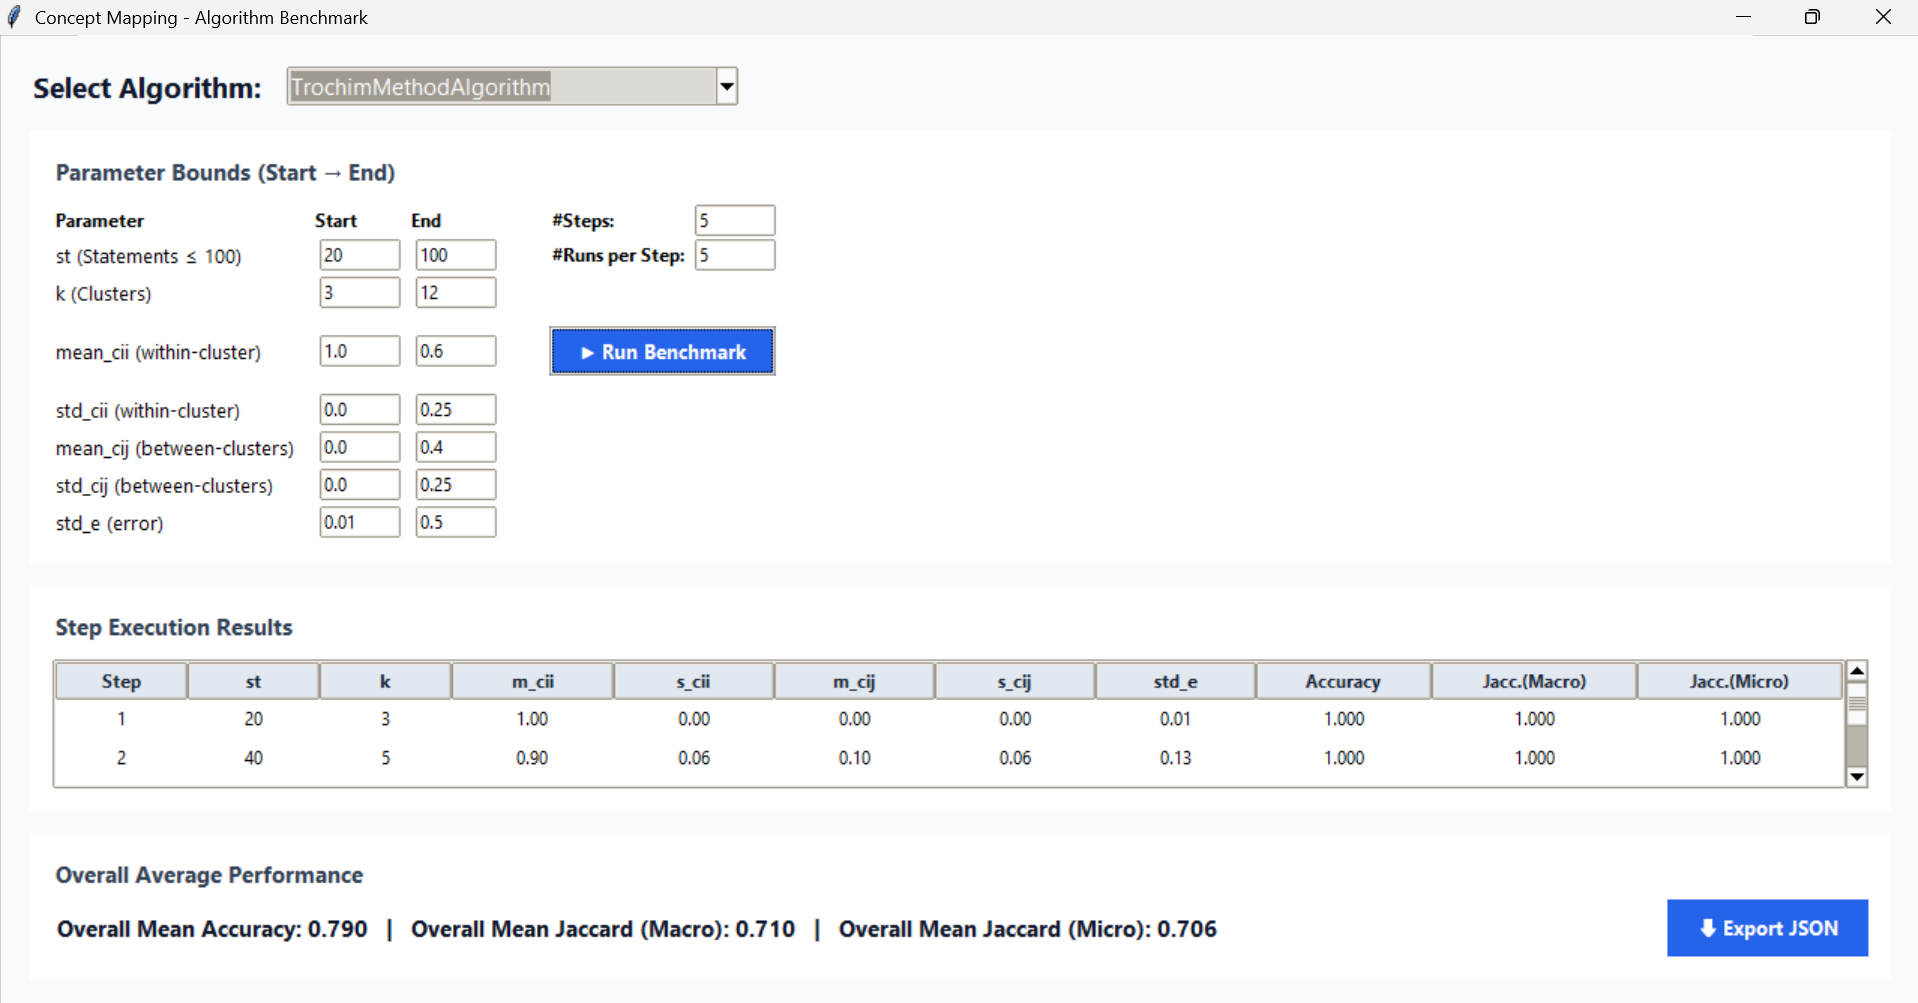
\includegraphics[width=0.9\textwidth]{figures/main_page_cmap.png}
    \caption{Benchmark interface used to run an algorithm across a parameterized difficulty trajectory and inspect step-level and overall performance.}
    \label{fig:benchmark-gui}
\end{figure}

The command $\texttt{python main.py --mode math}$ opens the mathematical visualization interface (see Figure \ref{fig:math-mode}). This mode is a helper tool for understanding how the true model is created. It allows the user to generate or manually enter \(Z\), generate \(C\), \(S_0\), \(E\), and \(S\), inspect the matrices, expand them, and visualize either \(S_0\) or \(S\) using non-metric MDS.

\begin{figure}[h!]
    \centering
    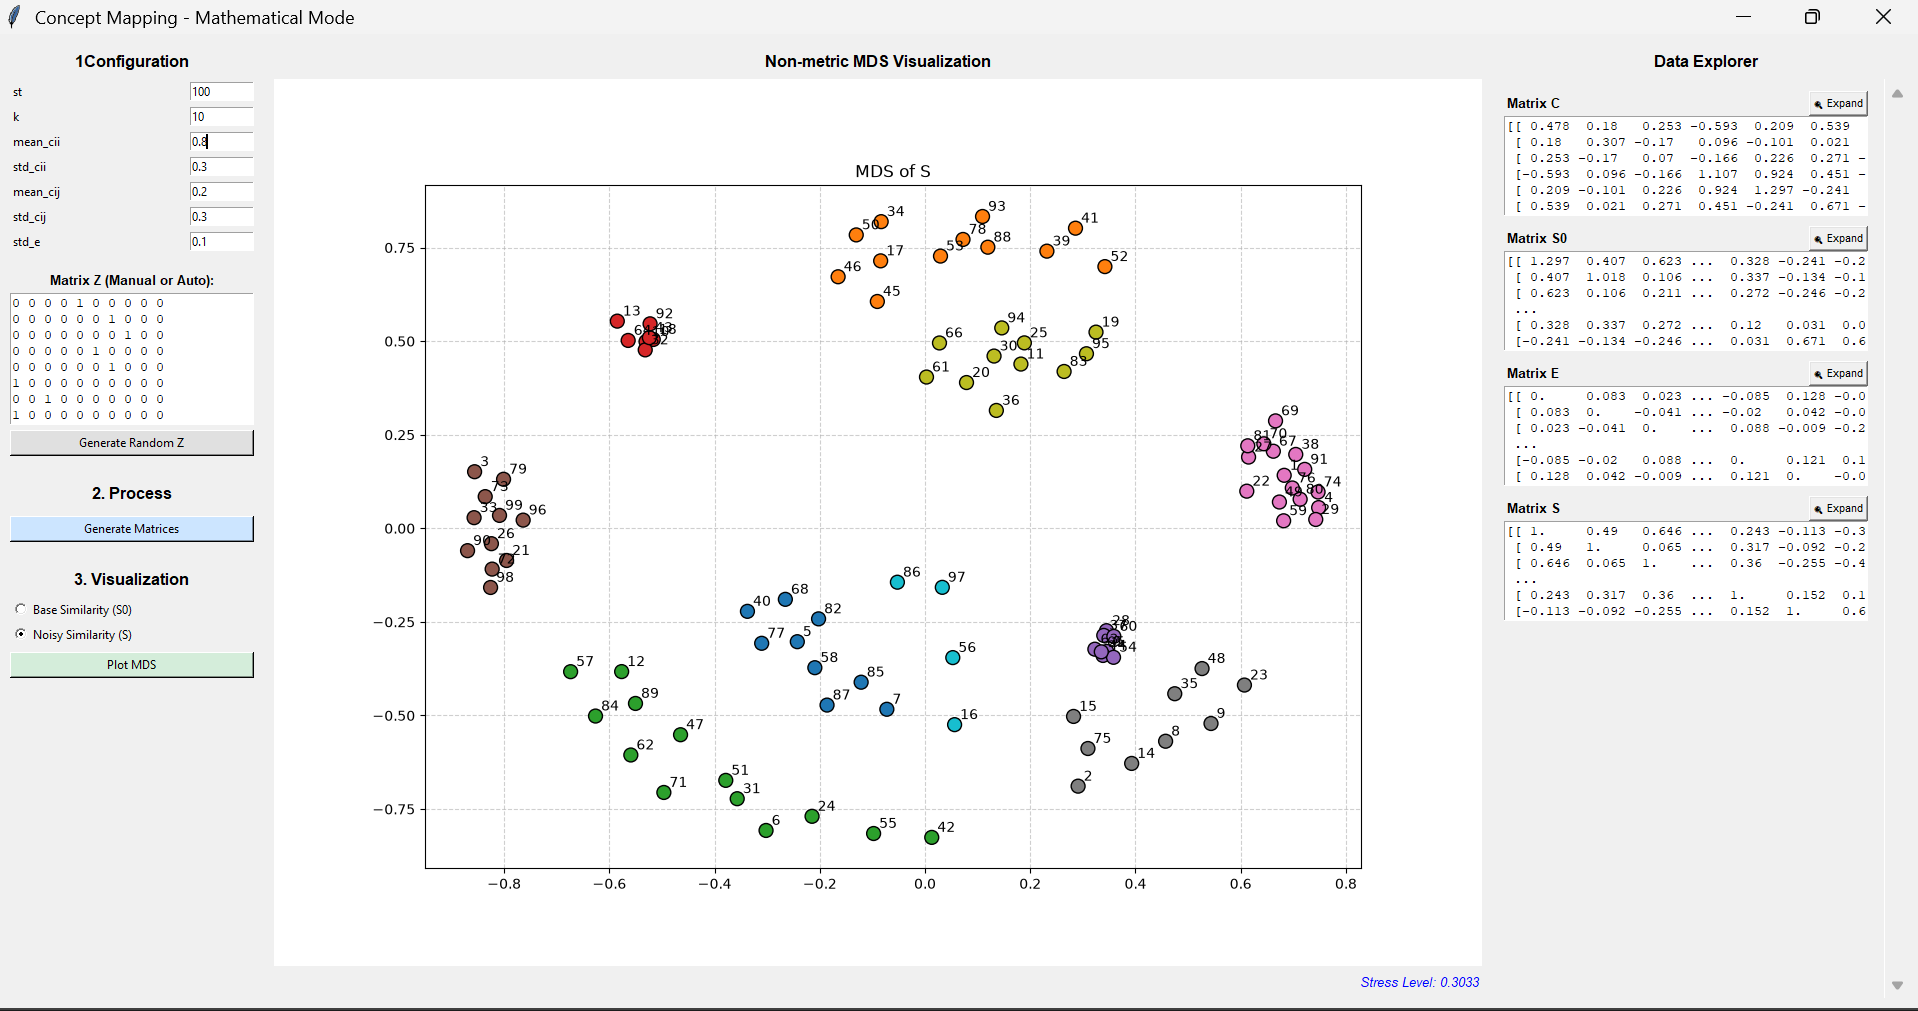
\includegraphics[width=0.9\textwidth]{figures/math_page_cmap.png}
    \caption{Mathematical mode used to inspect the generated matrices and visualize the geometry induced by \(S_0\) or \(S\).}
    \label{fig:math-mode}
\end{figure}

\section{Annex: Analytical Examples}

The following examples use the same ground-truth assignment matrix \(Z\), but different cluster similarity matrices \(C\). This shows that the same true partition can generate different statement-level similarity matrices depending on the assumed relationships between clusters.

\[
Z =
\begin{bmatrix}
1 & 0 & 0\\
0 & 1 & 0\\
0 & 0 & 1\\
1 & 0 & 0\\
0 & 1 & 0
\end{bmatrix}.
\]

Thus, statements \(1\) and \(4\) belong to cluster \(1\), statements \(2\) and \(5\) belong to cluster \(2\), and statement \(3\) belongs to cluster \(3\).

\subsection*{Example 1: Orthogonal Cluster Structure}

Let
\[
C_1 =
\begin{bmatrix}
1 & 0 & 0\\
0 & 1 & 0\\
0 & 0 & 1
\end{bmatrix}.
\]

Then
\[
S_{0,1}=ZC_1Z^\top
=
\begin{bmatrix}
1 & 0 & 0 & 1 & 0\\
0 & 1 & 0 & 0 & 1\\
0 & 0 & 1 & 0 & 0\\
1 & 0 & 0 & 1 & 0\\
0 & 1 & 0 & 0 & 1
\end{bmatrix}.
\]

In this case, statements in the same cluster have similarity \(1\), and statements in different clusters have similarity \(0\). The resulting matrix represents an easy clustering problem.

\subsection*{Example 2: Correlated Cluster Structure}

Let
\[
C_2 =
\begin{bmatrix}
0.9 & 0.2 & 0.3\\
0.2 & 0.9 & 0.1\\
0.3 & 0.1 & 0.9
\end{bmatrix}.
\]

Then
\[
S_{0,2}=ZC_2Z^\top
=
\begin{bmatrix}
0.9 & 0.2 & 0.3 & 0.9 & 0.2\\
0.2 & 0.9 & 0.1 & 0.2 & 0.9\\
0.3 & 0.1 & 0.9 & 0.3 & 0.1\\
0.9 & 0.2 & 0.3 & 0.9 & 0.2\\
0.2 & 0.9 & 0.1 & 0.2 & 0.9
\end{bmatrix}.
\]

After enforcing the framework convention \(S_{ii}=1\), this becomes:

\[
\widetilde{S}_{0,2}
=
\begin{bmatrix}
1 & 0.2 & 0.3 & 0.9 & 0.2\\
0.2 & 1 & 0.1 & 0.2 & 0.9\\
0.3 & 0.1 & 1 & 0.3 & 0.1\\
0.9 & 0.2 & 0.3 & 1 & 0.2\\
0.2 & 0.9 & 0.1 & 0.2 & 1
\end{bmatrix}.
\]

Here the same \(Z\) is preserved, but the relationships between clusters are no longer orthogonal. Therefore, the generated statement-level matrix contains non-zero between-cluster similarities. This is still structured, but it is less perfectly separated than the first example.

\end{document}
